\documentclass[11pt]{book}
\usepackage{amssymb,amsmath}
\usepackage{minitoc}
\usepackage{hyperref}
\usepackage{graphicx}


\title{Notes on BIOMEDE 211, or: \\ Circuits, Systems, \& Signals \\ in Biomedical Engineering}
\author{Barry Belmont}

\begin{document}
\frontmatter
\maketitle
\dominitoc
\tableofcontents


\newpage 
\section{How can I print off and use this document?}
Frankly, in just about any way that’s useful to you. I am going to try something here, where I will try to make more or less the entirety of the notes associated with the Winter 2019 semester of BIOMEDE 211, ”Circuits, Systems, and Signals in Biomedical Engineering”, to you, dear reader.
\\
Please don’t plagiarize this. If you were raised right, you ought to know what that is. If you’d like my judgment on any sort of action, my opinions can be laid bare.
\\
The first assignment I am giving you (worth 4\% of your grade and which must be completed by the end of the semester) is to figure out where this document is located online, download it, print it off, sign your name to it, and get it to me. If you know who I am, I would expect a competent engi- neer to find that without much to-do about it. Start with Google, go from there. Further, for those in the class, BIOMEDE 211, Winter 2019, you must join Github and make at least four substantive contributions to this repository. The term all you engineers (and lawyers) can’t wait to parse is “substantive” to which I will always enter a judgment which I deem final in this class, and I am ever in favor of beneficence over stricture. So, just help out the class in a way you think is helpful and watch those around you do the same. Failure to contribute to this living document by the end of the semester for those in this class will result in a loss of up to 4\% of one's total grade outright.

\newpage
\section{How to contribute to GitHub}
Follow these general steps to propose a change to this online document:
\begin{enumerate}
\item Create a GitHub account
\subitem This should be rather self-explanatory. Use your e-mail account and verify it to be able to edit. You should proceed with the following steps while logged onto your account.
\item Find Dr. Belmont's GitHub page and go to the biomede-211-w19 repository (``repo''). Then click on the biomede-211-w19.tex file.
\item Edit the file
\subitem You will find a small pencil icon on the right side of the page. Click on this to create your own branch (``forking''), and edit the file as you wish.
\item Propose file change
\subitem After making your changes, you should scroll to the bottom of the page, find the message box that says, 'Propose file change', and fill it out. The first line should say what you have updated and can be explained in the description.
\item Create pull request
\subitem After finishing your file, you will be brought to a page that displays what you have modified on the original document. Press the green `Create pull request' button to let Dr. Belmont know that you want to create a change. Once he has approved via his own GitHub account, your changes should now be in the updated master branch!
\end{enumerate}

\newpage



\section{Who comprises this class and how can they be reached?}
\subsection{The Captain at the helm}
Barry Belmont \\ Wednesdays 11:00 a.m. | 1:00 p.m., 2130 LBME \\ belmont@umich.edu \\
\subsection{The A-Team}
Annabelle St. Pierre \\ Wednesdays 5:00 p.m. | 6:30 p.m., UGLI basement \\ astpierr@umich.edu \\
\\
Alice Tracey \\ Wednesdays 4:00 p.m. | 5:00 p.m., UGLI basement \\ atracey@umich.edu \\

\subsection{You, yourselves}
In this class, we will be learning a lot from each other. You are encouraged to learn from one another. You are encouraged to talk to one another. You are are encouraged to share ideas and at times data. You are not encouraged and are hereby expressly forbidden to submit the work of another as your own. If you get help from others, you will put their name on it somewhere. Too much of this and you are committing plagiarism, not enough and you are committing fraud. Please be honest and let's all learn together.



\newpage
\section{The policies of this class}


\mainmatter
\setcounter{page}{1}



\part{Circuits}



\chapter{I. Potential, current, energy, conservation}
01/10/2019
\minitoc



\section{What is electricity?}

\begin{enumerate}
	\item A form of energy resulting from the existence of charged particles 
	\item The physical phenomena arising from the existence, presence, and motion of charged particles
	\item Rather ill-defined in common vernacular – we will generally avoid its use
\end{enumerate}



\section{Charge}
 
\begin{enumerate}
	\item Charge is the property of matter that causes it to experience a force when placed in an electromagnetic field; measured in coulombs (C)
	\item 	Charges are found in nature in discrete, integral multiples of electronic charge: e  = -1.602 x $10^{-19}$ C (the charge of one electron)
	\item \textbf{How many electrons are needed to form one coulomb?} (What is the weight of all those electrons?) 
	\item One byte is eight bits. Bits are essentially a single electron stored in a transistor. \textbf{If we were to take all the electrons from one terabyte of well distributed information (equal number of ones and zeros), how many coulombs would we have?}
\end{enumerate}


\section{Current}
\begin{enumerate}
	\item The time rate of change of charge – charges (charged particles) in motion; measured in amperes; defined mathematically as
	\begin{equation}
	\label{i=dqdt}
		i := dq/dt
	\end{equation}
	where $i$ is current, $q$ is charge, and $t$ is time
	
	\item Conversely, the total charge transferred over time can be expressed as 
	\begin{equation}
	\label{q=it}
		Q := \int_{t_0}^{t}i dt
	\end{equation}

	\item 1 ampere is equal to 1 coulomb/second
	\item Direct current, ``DC'', is current that remains constant with time
	\item Alternating current, ``AC'', is current that varies sinusoidally with time
\end{enumerate}


\subsection{The directionality of current}
Ultimately, the direction in which we say "current" flows is largely arbitrary. As arbitrary as choosing one type of charge and calling it ``positive'' and another ``negative''. The reason it doesn't matter is that the only consequence of having chosen a ``wrong direction'' for the current in a given analysis is that we have to switch the sign of the value. Thus, 3 amps in one direction is \textit{the exact same thing }as -3 in the opposite direction.
\begin{enumerate}
	\item Thanks to Benjamin Franklin we say that current is 
	\subitem i.	\textbf{Positive in the direction in which positively charged particles flow} and 
	\subitem ii.	\textbf{Negative in the direction in which negatively charged particles}
	\subitem iii.	We also now know that current results primarily from the movement of negatively charged particles (electrons) and therefore our convention is “wrong” in one sense, though convenient and entrenched enough that we’re not liable to change it in our life time (besides, the math comes out the same, and the actual flow of electrons will only matter to us in a few special circumstances, diodes)
\end{enumerate}


\subsection{The at times deadly serious nature of current}
Much of the point of learning this material here is its eventual application by our hands or by the hands of those we work with. Before we put any of this stuff in our hands, we should probably know what is and is not safe.
\begin{enumerate}
	\item 1 mA, you will feel
	\item 10 mA, you will really feel
	\item 100 mA, you will likely die
	\item 1000 mA, you will definitely die
\end{enumerate}


\subsection{The ``speed'' of current}
A possible misconception is that the electrons inside a wire travels at the speed of light. The speed of current is actually relatively slow. If one were to imagine an electron starting at the wire next to a light switch in an average classroom, it would take a very long period of time for it to travel to the light itself. The light's immediate reaction to a switch is due to a ''hose effect''; the electrons inside the wire push other electrons in the direction opposite to the [conventional] current. This cascade of electrons is what happens close to the speed of light, not the electron movement itself.

\begin{enumerate}
	\item T\textbf{he \textit{signal} of electrical current (that is electromagnetic radiation) travels anywhere between about 50-99\% the speed of light} (dependent on a number of conditions) depending upon the material through which it travels (based on a “dielectric” behavior known as permittivity)
	\item \textbf{The drift velocity of electrons} within a copper wire is ~25 $\mu$m/s, so how does anything ever turn on?
	\item \textbf{The hose effect} - The electrons at the light switch will almost certainly never pass through a light bulb, but they will move around and bump into their neighbors which bump into their neighbors which bump into their neighbors, etc., until it causes the electrons nearest the light to pass through. This is how water at a spigot is able to push water at the end of a hose.
\end{enumerate}



\section{Potential (difference)}
\begin{enumerate}
	\item The amount of work needed to move a unit of (positive) charge from a reference point to another point [without producing an acceleration]).
	\item Potential is measured in ``volts'' and is often called ``voltage''. In this class we will endeavor to avoid such a term as it can be very confusing to talk about potential as if there were such a \textit{thing} as voltage.
	\item Defined as 
	\begin{equation}
		v:= \frac{dw}{dq}
	\end{equation}
	\item Potential describes the \textit{potential} to do something. Increasing the potential is akin to increasing the height of a cliff. The height does not \textit{do} anything other than increase what can be done on the drop. If potential is the cliff's height, charge would be pebbles you'd drop off the side, and current describes how fast those pebble fall.
	\item In this class, and for the vast vast majority of electrical engineering work, we care about the \textit{difference} in potential. One element held at 100 billion volts and another held at 100 billion + 1 volts has a \textit{potential difference} of 1 V, which is less than a single AA battery.
	\item Some typical voltages to be aware of
	\subitem \textbf{Consumer level batteries} (AA, AAA): 1.5 V (DC); 9 V (DC) 
	\subitem \textbf{Car batteries}: 12 V (DC)
	\subitem \textbf{The ``mains''} (levels provided by power companies to consumers): 110-120 V (AC) and 220-240 V (AC) in America
	\subitem \textbf{Power transmission lines}: 110-1200 kV (AC), transformers are used to step up and down the potential before used by consumers
\end{enumerate}



\section{Power}
\begin{enumerate}
	\item The time rate of expending or absorbing energy.
	\item Quantifies the rate of energy transfer.
	\item Mathematically:
	\begin{equation}
		p = \frac{dw}{dt} = \frac{dw}{dq}\cdot\frac{dq}{dt} = v\cdot i
	\end{equation}
	\item Measured in watts: 1 W = 1 $\frac{\text{J}}{\text{s}}$ = 1 $\frac{\text{N}\cdot \text{m}}{\text{s}}$ = 1 $\frac{\text{kg}\cdot \text{m}^2}{\text{s}^3}$ = 1 V $\cdot$ 1 A
	\item \textbf{Passive sign convention}: If current enters through the positive terminal of an element, $p = +vi$; if current enters through the negative terminal of an element, $p = -vi$.
\end{enumerate}



\section{Energy}
\begin{enumerate}
	\item The capacity to do work.
	\item Measured in joules.
	\item $E = \int\frac{dw}{dt}dt \rightarrow$ power x time
	\item J = $\frac{\text{kg}\cdot\text{m}^2}{\text{s}^2}$ = N $\cdot$ m = Pa $\cdot$ m$^3$ = W $\cdot$ s = C $\cdot$ V
\end{enumerate}



\section{Conservation}
Here, as elsewhere, things will be conserved. In electrical circuits there are two laws of conservation that will matter most for us:
\begin{enumerate}
	\item \textbf{The Conservation of Mass.} The conservation of mass means that no mass can be added to or removed from a circuit without being accounted for. Put differently, in a closed system (the type we will concern ourselves with here) no mass is added or removed.
	\subitem In electrical circuits, the mass we care the most about are the charges whipping around. Thus, for us, \textit{the amount of charge within a circuit must remain constant.}
	\item \textbf{The Conservation of Energy.} The conservation of energy means that no energy can be added to or removed from a circuit without being accounted for. Put differently, in a closed system (the type we will concern ourselves with here) no energy is added or removed.
	\subitem In electrical circuits, the energy we care the most about is the potential provided by sources and depleted by other elements in the circuits. Thus, for us, \textit{the sum of potentials within a circuit must equal zero.} 
\end{enumerate}

In evaluating circuits, the main focus of the first third of this class, it will be the application of these two conservative laws that will enable us to ``solve'' them. That is, by understanding (1) how energy is generated and used and (2) how charges move around in closed loops (``circuits'') we will be able to predict the behavior of the myriad electrical systems which may cross our paths.


 
\newpage



\section{Worksheet}

\subsection{Problem 1, constant charge through a cross-section}
How much charge passes through a cross-section of a conductor in 60 seconds if a DC current value is measured at 0.1 mA?
\textbf{Solution}


\subsection{Problem 2, arbitrary charge through a cross-section}
Determine the total charge entering a terminal between $t = 0$ seconds and $t = 10$ seconds if the current (in amps) passing through is
\begin{equation}
	i(t) = \frac{1}{\sqrt{5t+2}}. 
\end{equation} 
\textbf{Solution}


\subsection{Problem 3, a "tera"ble puzzle}
Approximately how much current is necessary to transmit one terabyte of information in an hour?
\textbf{Solution}


\subsection{Problem 4, power necessary to run a pacemaker}
A cardiac pacemaker will provide approximately 5,000 J of energy over 5 years. Determine the capacity of a 5 V lithium battery necessary to drive this pacing such that only 40\% of its energy is spent over that time.
\textbf{Solution}


\subsection{Problem 5, energy needed to excite a neuron}
A colleague of yours has been in their lab ginning up new neurons. You, as their resident electrical expert, are tasked with determining the energy consumed by the cell. If the current and voltage variations are found to be functions of time ($t \geq 0$)
\begin{eqnarray}
	i(t) = 3t \\
	v(t) = 10 e^{6t}
\end{eqnarray}
determine the energy consumed between 0 and 2 ms.
\textbf{Solution}


\subsection{Problem 6, a thump to the chest}
(a) A typical defibrillator delivers 200-1000 V in less than 10 ms. How much current is needed to deliver 120, 240, and 360 Joules?
\\
(b) A human heart ways about 300 grams. From approximately how high of a cliff would one have to drop a heart such that the impact was equivalent to the energy delivered to someone's chest from a defibrillator?
\textbf{Solution}



\chapter{An introduction: II. Circuit elements}
\minitoc
01/15/2019
\section{Active v. passive}
\begin{enumerate}
	\item Active elements are capable of generating energy while passive components cannot
	\item \textbf{Active}: generators, batteries, operational amplifiers, ``sources''
	\item \textbf{Passive}: resistors, capacitors, inductors, i.e., most circuit elements
\end{enumerate}

\section{Ohm's Law and what it means}

Ohm's Law is concerned with the relationship between voltage, or potential difference, and current across a conductor.  The potential difference across a conductor is proportional to the current flowing thorugh the conductor with the proportionality constant being denoted as R, or resistance.  This can be expressed as:

	\begin{equation}
	\label{V=iR}
		V := iR
	\end{equation}
	
This essentially states that the drop in potential across the conductor, or resistor, is equivalent to the current flowing through the conductor and its resistance.  When considering impedance, the equation can be modified to state:

	\begin{equation}
	\label{V=iZ}
		V := iZ
	\end{equation}

\section{Sources}
\begin{enumerate}
	\item \textbf{An ideal independent source} is an active element that provides a specified value of potential or current, regardless of other circuit elements.
	\subitem Batteries and power supplies may be approximated as ideal potential sources.
	\item \textbf{An ideal dependent (or controlled) source} is an active element in which the source quantity is controlled by another quantity (such as potential, current, temperature, measured resistance, etc.).
	\item \textbf{An ideal potential source} will produce any current required to ensure that the terminal voltage stated is satisfied.
	\item \textbf{An ideal current source} will produce any voltage required to ensure that the terminal current as stated is satisfied
	\item Symbols
	\subitem Voltage-controlled voltage source, VCVS
	\subitem Current-controlled voltage source, CCVS
	\subitem Voltage-controlled current source, VCCS
	\subitem Current-controlled current source, CCCS 
\end{enumerate}

\section{Resistors}
\textbf{Resistors} are electrical (circuit) elements that resist the flow of electric charge (current); passive two-terminal components that implement a defined/``constant'' resistance; meant to reduce current flow and change potential

\subsection{Resistance, $R$}
\begin{enumerate}
	\item \textbf{Resistance} is the physical property describing an element's ability to resist current and is most often represented by $R$
	\item Resistance is measured in ``ohms'', $\Omega$, which is equivalent to 1 V/A
	\item Resistance is one half of a broader physical phenomenon known as \textbf{``impedance''} - the property describing an element's ability to \textit{impede} current. Impedance is typically represented by $Z$, which we'll explore more thorough in a bit.
\end{enumerate}

\subsection{Resistivity, $\rho$}
\begin{enumerate}
	\item The resistance of an element (such as a resistor) depends on three things: 
	\subitem \textbf{Resistivity}, $\rho$, of the material comprising the element, which is the \textit{material}'s ability to resist the flow of charges; measured in ohm-meters
	\subitem \textbf{Length}, $l$, of the element; measured in meters
	\subitem \textbf{Area}, $A$, of the cross-section of the element; measured in m$^2$
	\subitem Such that $R = \rho\frac{l}{A}$
	\subsubitem What units are we left with?
	\subsubitem What are the effects of length and area?
	\item \textbf{Materials with low resistivity} are generally called (and treated as) ``conductors'' as they are able to more effectively \textit{conduct} the motion of electrical charges than materials with high resistivity
	\item \textbf{Materials with very high resistivity} are generally used as ``insulators'' as they prevent the flow of current through them and thus \textit{insulate} the current within prescribed bounds, such as with a copper wire with plastic wrapped around it.
\end{enumerate}

Here is a link to a video that further explains the concepts of resistivity and resistance: \url{<https://www.youtube.com/watch?v=4rsswT_Rv1M>}.

\subsection{Conductance}
\begin{enumerate}
	\item The inverse of resistance is conductance, $G$, which describes the ability of an element to conduct current
	\item Measured in Siemens
	\item Allows us express Ohm's law slightly differently, $i = Gv$, which says that the current generated through an element by a potential is directly proportional to some constant, namely conductance.
	\item The material specific property \textbf{conductivity}, $\sigma$ is measured in S/m
\end{enumerate}

\section{Capacitors}
\begin{enumerate}
	\item Passive two-terminal components that store energy in an electric field; introduces capacitance to a circuit.
	\item Can be thought of as two conductive plates sandwiching a ``dielectric'' material. Essentially it is two ``conductors'' separated by a ``non-conductive region''.
	\item When a capacitor is attached across a source, an electric field develops across the dielectric causing a net positive charge to collect on one conductor and a net negative charge to collect on the other.
	\item We can define the capacitance of an element mathematically as 
	\begin{equation}
		C = Q/V
	\end{equation}
	where $C$ is capacitance in farads, $Q$ is positive or negative charge on each conductor, and $V$ is the potential between them
	\item We can also represent capacitance by the voltage-based rate of charge accumulation: $C = dQ/dV$.
\end{enumerate}

\subsection{Its time varying behavior}
Unlike resistors, capacitors have a \textit{time-varying} element to that. That is, since $C = Q/V$, $V = Q/C$.

If we then recall Equation \ref{q=it}, we can write the time-dependent potential relationship of a capacitor
\begin{equation}
	V(t) = \frac{Q(t)}{C} = \frac{1}{C}\int_{t_0}^{t} i(\tau) d\tau + V(t_0)
\end{equation}

We can also recall\footnote{We could also take the derivative of the equation preceding this one and do a little rearrangement. As it turns out, these physical relationships are rather codified and thus can be gotten out by any number of means.} Equation \ref{i=dqdt}, and represent the time-dependent current relationship as
\begin{equation}
	I(t) = \frac{dQ(t)}{dt} = C\frac{dV(t)}{dt}
\end{equation}

\subsection{Charge accumulation}
\begin{enumerate}
	\item While charges accumulate on a capacitor, no current flows \textit{through} the capacitor.
	\item \textbf{Well, then why use them? After awhile won't the current just stop?} Yes, indeed it will -- in a DC circuit!
	\item The capacitor will become ``charged'' over time, eventually reaching the same potential as that established across it, e.g., by a source. Since potential only ever travels down potential gradients, if the capacitor and the source (say, a battery) are at the same potential, no current will flow.
	\item Thus, a fully charged capacitor will act as an ``open'' circuit, while an uncharged capacitor will act as a ``short'' circuit.
\end{enumerate}

\subsection{A simple example}
If we consider Ohm's law for a simple RC circuit (one in which a source, a resistor, and a capacitor are in series), we can describe the system by

\begin{align}
	V_0 &= v_{R}(t) + v_{C}(t) \\
	V_0 &= i(t)R + \frac{1}{C}\int_{t_0}^t i(\tau)d\tau
\end{align}
Taking the derivative of both sides:
\begin{align}
	0 &= R\frac{di(t)}{dt} + \frac{1}{C}i(t) \\
	0 &= RC\frac{di(t)}{dt} + i(t) \\
	i(t) &= \frac{V_0}{R}\cdot e^{-t/RC} \\
	v(t) &= V_0\left(1 - e^{-t/RC}\right) \\
	Q(t) &= C\cdot V_0\left(1 - e^{-t/RC}\right)
\end{align}


\section{Inductors}

\begin{enumerate}
	\item Passive two-terminal components that store energy in a magnetic field
	\item Can be thought of as an insulated wire wound into a coil around a core (which may either be filled with a material or left open to the environment)
	\item Behavior can be modeled as $L = \frac{\Phi}{I}$, where $L$ is the inductance, $\Phi$ is the magnetic flux generated by a current, $I$.
	\item By Faraday's law of induction, voltage induced by a change in magnetic flux through a circuit is
	\begin{equation}
		v = \frac{d\Phi}{dt}
	\end{equation}
	which we can rewrite as
	\begin{equation}
		v = \frac{d}{dt}(Li) = L\frac{di}{dt}
	\end{equation}
	\item In this class, at this level, and for most biomedical applications you're liable to experience in your tenure, you will not work extensively with inductors. However, you should be able to recall at least this much at a moment's notice to be able to ascertain a system's behavior.
\end{enumerate}




\section{Impedance}

\begin{enumerate}
	\item The measure of opposition a circuit element presents to a current when a potential is applied. (It is measured in ohms.)
	\item It is ``complex'' in two sense of the term. First, the actual phenomenon itself comprises complex numbers; that is, there is both a ``real'' and an ``imaginary'' component.
	\subitem \textbf{The real component} is known as resistance, $R$
	\subitem \textbf{The imaginary component} is known as reactance, $X$
	
	Impedance can be represented as a combination of either
	\subitem \textbf{Resistance and reactance}: $\mathbf{Z} = R + \jmath X$, where $\mathbf{Z}$ is impedance, $R$ is resistance, and $X$ is reactance, or
	\subitem \textbf{Magnitude and phase}: $\mathbf{Z} = |Z|e^{\jmath \theta}$, where $|Z|$ is the magnitude of the impedance vector, $\mathbf{Z}$, and $\theta$ is the phase of said vector (i.e., the delay between current and potential). Phase, $\theta$ is equivalent to $\tan^{-1}(X/R)$
	\item Impedance is also complex in the sense that it is complicated. The impedance of an object is a factor of many parameters including permittivity, geometry, quantum states, thermal stability, etc. Let us not view this sort of complexity as an impediment to our understanding of impedance.
	\item The inverse of impedance is \textbf{admittance}, $Y$, and comprises a real component, \textbf{conductance}, $G$, (which is the inverse of resistance) and an imaginary component, \textbf{susceptance}, $B$ (which is the inverse of reactance). (It is measured in Siemens.)
	\subitem $\mathbf{Y} = G + \jmath B$
\end{enumerate}

\subsection{A quick note on ``imaginary'' numbers}
The term ``imaginary'' is an unfortunate name for an excellent mathematical tool. All the imaginary operator -- in this class represented by $\jmath = \sqrt{-1}$ -- is is a type of number ``orthogonal'' to our ``real'' numbers. Imaginary numbers are no less ``real'' than real numbers. Unfortunately, they aren't necessarily the most intuitive to our little mammalian brains and thus we must be trained to work with them. However, as we will see in this class, they can be quite useful.

\section{Equivalent impedance}
\begin{enumerate}
	\item It will often be more convenient to think about the impedance which a component burdens a system with (or the conductance which it affords) rather than its resistance. \textbf{Therefore, we need to begin to think in terms of equivalent impedances as we start to evaluate circuits.}
	\item Recall Ohm's law 
	\subitem \textbf{Resistors}, $v = iR \qquad \qquad \rightarrow Z_{eq,R} = R$
	\subitem \textbf{Capacitors}, $v = \frac{1}{C}\int i dt \quad \rightarrow Z_{eq,C} = \frac{1}{\jmath \omega C}$
	\subitem \textbf{Inductors}, $v = L\frac{di}{dt} \quad \qquad \rightarrow\jmath \omega L$
	
	I want to plant a flag here for you to notice the relationship between the $\jmath \omega$ terms from the capacitor and inductor and the corresponding derivative and integral forms of current in the Ohm's law representation. This will become very important once we get into the Laplace and Fourier transforms.
	\item We must also recognize that few will be the circuits comprising but a single element. As such, we should know how to find the equivalent impedance of many elements.
\end{enumerate}

\subsection{Impedances in general}
\textbf{Series}
\begin{equation}
	\label{zeq,ser}
	Z_{eq,series} = Z_1 + Z_2 + Z_3 + ...
\end{equation}
\\
\textbf{Parallel}
\begin{equation}
	\label{zeq,par}
	\frac{1}{Z_{eq,parallel}} = \frac{1}{Z_1} + \frac{1}{Z_2} + \frac{1}{Z_3} + ...
\end{equation}
\\
\textbf{A special case to remember}. When dealing with only two elements:
\begin{equation}
	\label{zeq,two}
	Z_{eq} = \frac{Z_1\cdot Z_2}{Z_1 + Z_2}
\end{equation}

\subsection{Resistors}

\textbf{Series}
\begin{equation}
	\label{req,ser}
	R_{eq,series} = R_1 + R_2 + R_3 + ...
\end{equation}
\\
\textbf{Parallel}
\begin{equation}
	\label{req,par}
	\frac{1}{R_{eq,parallel}} = \frac{1}{R_1} + \frac{1}{R_2} + \frac{1}{R_3} + ...
\end{equation}


\subsection{Capacitors}
\textbf{Series}
\begin{equation}
	\frac{1}{C_{eq,series}} = \frac{1}{C_1} + \frac{1}{C_2} + \frac{1}{C_3} + ...
\end{equation}
\\
\textbf{Parallel}
\begin{equation}
	C_{eq,parallel} = C_1 + C_2 + C_3 + ...
\end{equation}

\subsection{Delta-Wye ($\Delta$-$Y$) transformations}
\textbf{Going from Delta to Wye}
\begin{align}
	Z_1 = \frac{Z_b Z_c}{Z_a+Z_b+Z_c} \\
	Z_2 = \frac{Z_a Z_c}{Z_a+Z_b+Z_c} \\
	Z_3 = \frac{Z_a Z_b}{Z_a+Z_b+Z_c}
\end{align}
\\
\textbf{Going from Wye to Delta}
\begin{align}
	Z_a = \frac{Z_1Z_2 + Z_2Z_3 + Z_1Z_3}{Z_1} \\
	Z_b = \frac{Z_1Z_2 + Z_2Z_3 + Z_1Z_3}{Z_2} \\
	Z_c = \frac{Z_1Z_2 + Z_2Z_3 + Z_1Z_3}{Z_3} \\
\end{align}

\subsection{A few examples}
\textbf{Example 1}
Find the equivalent resistance, if a resistor $R_1 = 10 \text{ k}\Omega$ is connected in parallel to $R_2 = 3.3 \text{ k}\Omega$.

\textit{Solution}. $R_{eq} = \frac{R_1 \cdot R_2}{R_1 + R_2} = \frac{(10)(3.3)}{10 + 3.3} = 2.48 \text{ k}\Omega$
\\
\\
\textbf{Example 2}
Find the equivalent resistance of three parallel-connected resistors of equal value. If $R = R_1 = R_2 = R_3 = 10 \text{ k}\Omega$, what's $R_{eq}$?

\textit{Solution}.
Recall, Equation \ref{req,par}
\begin{equation}
	\frac{1}{R_{eq}} = \frac{1}{R} + \frac{1}{R} + \frac{1}{R} \rightarrow 3R_{eq} = R \rightarrow R_{eq} = \frac{R}{3} \rightarrow R_{eq} = \frac{10k}{3} = 3.33 k\Omega
\end{equation}
\\
\\
\textbf{Example 3}
Four resistors are connected in parallel. $R_1 = 10 \text{ k}\Omega$, $R_2 = 1 \text{ k}\Omega$, $R_3 = 5 \text{ k}\Omega$, and $R_4 = 3 \text{ k}\Omega$. Calculate their equivalent resistance.
\begin{align}
	\frac{1}{R_{eq}} &= \frac{1}{R_1} + \frac{1}{R_2} + \frac{1}{R_3} + \frac{1}{R_4} \\
	\frac{1}{R_{eq}} &= \frac{1}{10k} + \frac{1}{1k} + \frac{1}{5k} + \frac{1}{3k} \\
	&= 612.3 \text{ }\Omega
\end{align}

\section{Grounds}
\begin{enumerate}
	\item A reference point in an electrical circuit from which potentials are measured
	\item A common return path within a circuit
\end{enumerate}


\section{Conductors}
\begin{enumerate}
	\item Allow from the transmission of electrical energy
	\item Serve to connect circuit elements
	\item Also known as wires and traces
	\item Within circuit schematics we must be mindful of ``junctions'' and ``jumps'' in conductors
\end{enumerate}


\section{Operational amplifiers}
\begin{enumerate}
	\item Active components that deliver the amplified difference between two of its terminals
	\item Will be discussed at length in the next class and along with resistors, capacitors, and sources, will be among the primary circuit components we work with
\end{enumerate}


\section{Diodes}
Two-terminal circuit elements that allow current to flow only in one direction

\section{Switches}
Make/break/change circuit paths (thereby diverting current or removing potential)

\begin{enumerate}
	\item Single pole, single throw, SPST
	\item Single pole, double throw, SPDT
	\item Double pole, single throw, DPST
	\item Double pole, double throw, DPDT
\end{enumerate}


\section{Transistors}


\section{Transformers}
\begin{enumerate}
	\item Transfer electrical energy between circuits using induction
	\item Allows for the effective transmission of power and the stepping up/down of potential
	\item Crucial for the transmission, distribution, and utilization of AC
\end{enumerate}

\newpage
\section{Worksheet}
\subsection{Problem 1, expressing power in ohms}
Utilizing Ohm's law, express units of power to include ohms.

\textbf{Solution}


\subsection{Problem 2, a couple toaster based problems}
A toaster draws 2 A at 120 V. What is its resistance?

\textbf{Solution}
\\
\\
How much current is drawn by a toaster with a resistance of 10 $\Omega$ at 110 V?

\textbf{Solution}

\subsection{Problem 3, currently conducting power}
In the circuit shown, calculate the current, $i$, the conductance, $G$, and the power, $p$.

\textbf{Solution}


\subsection{Problem 4, conductance of a sodium channel}
Conductance ($G$/$A$) of a sodium channel of a cell membrane at a specific time is 10 mS/cm$^{2}$. If the channel length as 100 nm, what is its conductivity?

\textbf{Solution}


\subsection{Problem 5, resistance of a simple tissue}
Determine the resistance of a homogenous and isotropic tissue with a cross-sectional area which can be described by the functions $y = 8 - x^2$ from $x = -2$ cm to $x = +2$ cm, a length of 10 cm (parallel to the z-axis), and a resistivity of 80 $\Omega$m.

\textbf{Solution}




\chapter{An introduction: III. Operational amplifiers}
01/17/2019 
\minitoc

\section{Some details}
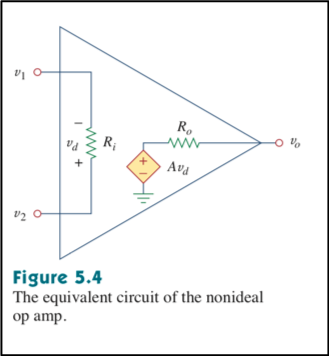
\includegraphics[width=0.5\textwidth]{figures/op-amp1}
\\
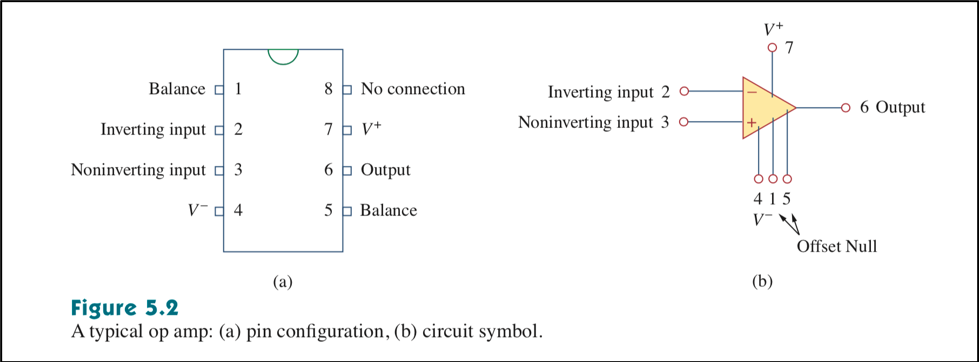
\includegraphics[width=\textwidth]{figures/op-amp2}

\begin{enumerate}
	\item Behaves like a voltage-controlled voltage source
	\item They can amplify, sum, subtract, multiply, differentiate, integrate
	\item They are active circuit elements
	\item Though they have somewhat more complicated internal workings, we typically represent them in electrical circuits as a triangle with three (sometimes five) very important terminals:
	\subitem An inverting input (— sign, typically represented up top for convenience, but it need not be)
	\subitem A non-inverting input (+ sign, typically on bottom)
	\subitem An output
\end{enumerate}

\section{Some rules}
There are \textbf{three important features of ideal operational amplifiers} that we must understand thoroughly. These are things worth stamping in your brain.

\begin{enumerate}
	\item \textbf{Infinite open-loop gain.} The ``A'' of the gain is infinitely large such that any difference in voltages $V_1$ and $V_2$ causes an enormously large output voltage. As much as is being supplied. (The real value of gain in most operational amplifiers is between $10^{5}$ and $10^8$.)
	\item \textbf{Infinite input impedance.} Current cannot travel between the inverting and non-inverting terminals. (Really, the impedance is between $10^5$ and $10^13$ ohms and is often signal dependent.)
	\item \textbf{Zero output impedance.} There is no loss transmitting a voltage difference to the output. (Really is about 10-100 ohms and is chip dependent.)
\end{enumerate}

\section{Some conveniences}
\begin{enumerate}
	\item With infinite input impedance, no current can flow into or out of the terminals and hence $i_1$ and $i_2$ are equal to 0.
	\item Since no current flows across the terminals, the terminals are at equal potential. Hence ``$v_1 = v_2$''.
\end{enumerate}

\newpage
\section{Some examples}

\subsection{Inverting amplifier}
We will apply the conservation of mass at this point to solve our equations.  This is among the simplest and most effective ways to add gain to a circuit. So much so that you will use it again and again and again in life and especially in labs

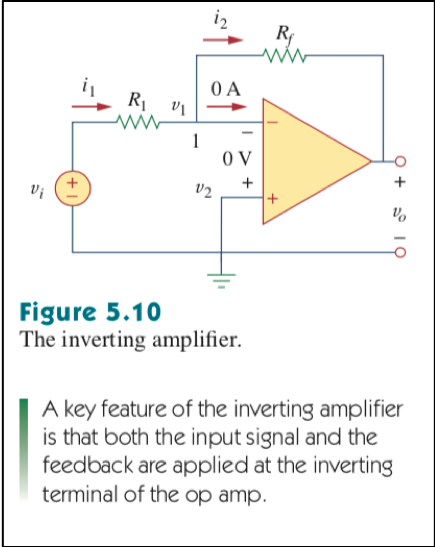
\includegraphics[width=0.5\textwidth]{figures/op-amp3}

We apply KCL at the node for v1
\begin{enumerate}
	\item I1 – i2 – i3 = 0
	\item I3 = 0
	\item I1 – i2 = 0
	\item I1 = i2
	\item I1 = (vi – v1)/R1
	\item I2 = (v1 - Vo)/Rf
	\item (vi – v1)/R1 = (v1 - Vo)/Rf
	\item V1 = V2 = 0
	\item Vi/R1 = -Vo/Rf
	\item Vo = -Rf/R1 * Vi
	\item R2/R1 is our gain, gain factor.
\end{enumerate}




\subsection{Non-inverting amplifier}
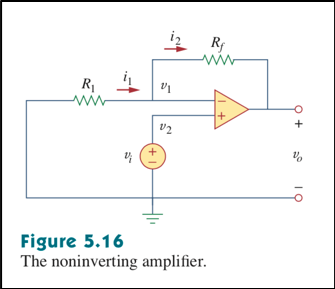
\includegraphics[width=0.5\textwidth]{figures/op-amp4}

Again, the name might imply what it does. It will amplify our input signal without inverting it.

We can again perform Nodal analysis.
\begin{enumerate}
	\item I1 – i2 – i3 = 0
	\item I3 = 0, since no current enters the non-inverting input
	\item I1 = i2
	\item (Vg – v2)/R1 = (v2 – Vo)/Rf
	\item –v2/R1 = (vi – Vo)/Rf
	\item Vo = (1 + Rf/R1) * Vi
\end{enumerate}



\subsection{Voltage follower}
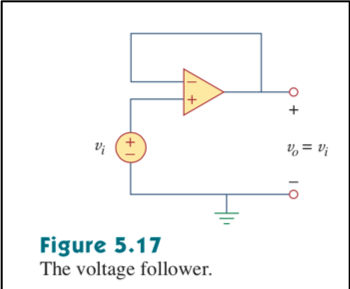
\includegraphics[width=0.5\textwidth]{figures/op-amp5.png}

What if we didn’t have any resistors? $\rightarrow$ Vi = v2 = v1 = Vo $\rightarrow Vi = Vo$


\subsection{Summing amplifier}
\subsection{Differential amplifier (as homework)}



\chapter{Circuit analysis: I. Nodal analysis}
01/22/2019
\section{Nodes and branches}
\begin{enumerate}
	\item \textbf{A branch} is any two-terminal element. (examples: Resistor, Capacitor, Wire, etc.)
	\item \textbf{A node} (junction) is a point of connection between two or more branches.
	\item \textbf{A loop} is any closed path within a circuit/ a closed path formed by starting at a node, going through a set of nodes, without crossing any node more than once.
	\subitem A loop is \textbf{independent} if at least one branch is not part of any other independent loop.
	\item \textbf{Fundemental theroem of Network topology} 
	\subitem # of branches = # of independent loops + # of nodes - 1
\end{enumerate}
\section{Kirchhoff's Laws} At any node or junction in a circuit the currents entering must equal the currents leaving.
	\subitem All current entering a node must sum to 0.
\subsection{Kirchhoff's Current Law} conservation of mass.
\subsection{Kirchhoff's Voltage Law} sum of potential differences around any closed network is 0.
\section{Nodal analysis}
\section{Solving simultaneous equations}
\subsection{Cramer's Rule}



\chapter{Circuit analysis: II. Mesh analysis; Homework I}
01/24/2019
\section{Mesh analysis}
\section{Steps of mesh analysis}
\section{Writing mesh equations directly in matrix form}



\chapter{Circuit analysis: III. Supernodes and supermeshes}
01/29/2019 – Lecture 6. 
\section{Nodal analysis with an independent current source}
\section{Nodal analysis with voltage sources, \textbf{Supernodes}}
\section{Nodal analysis with controlled sources}
\section{Mesh analysis with current sources}
\section{Mesh analysis with controlled sources, \textbf{Supermeshes}}



\chapter{Circuit analysis: IV. Circuit theorems}
01/31/2019 – Lecture 7. 
\section{Circuit theorems}
\section{Linearity}
\section{Superposition}
\section{Source transformation}
\section{Thevenin equivalents}
\section{Norton equivalents}
\section{Equivalents with dependents}



\chapter{Circuit analysis: V. When to choose between analyses}
02/05/2019 – Lecture 8. 

\chapter{A review of the material thus far; Homework II}
02/07/2019 – Lecture 9. 

\section{How to measure voltage and current}

\chapter*{Exam I}
02/12/2019



\part{Systems}



\chapter{The Laplace Transform: I. What it is and why it is important}
02/14/2019 – Lecture 10. 
\section{How do we know our world looks like this?}
\section{Euler's identity / Euler's formula}
\section{The Laplace transform}
\section{The Laplace transform of 1}
\section{The $s$-plane}
\section{The linearity of the Laplace transform}
\section{The Laplace transform of $e^{at}$}
\section{The Laplace transform of $dx/dt$}
\section{The Laplace transform in RLC circuits}
\subsection{Resistors}
\subsection{Inductors}
\subsection{Capacitors}
\subsection{RLC}
\section{Two important places, zeros and poles}



\chapter{The Laplace Transform: II. How to use it}
02/19/2019 – Lecture 11. 
\section{The inverse Laplace transform}
\section{The Laplace transform of $\sin$}
\section{The Laplace transform of $t^n$}
\section{Some applicability}



\chapter{Circuits as ODEs: I. First-order}
02/21/2019 – Lecture 12. 
\section{Source-free RC circuits}
\subsection{One resistor, one capacitor}
\subsection{Two or more resistors and/or capacitors}
\section{Source-free ``active'' circuits}
\section{First-order systems with sources}
\section{Several singular functions}
\subsection{Unit step function, $u(t-t_0) = 1, t>t_0$}
\subsubsection{The Laplace transform of the unit step function}
\subsection{Unit impulse function, $\delta(t) = du(t)/dt$}
\subsubsection{Its ``sifting'' abilities}
\subsubsection{The Laplace transform of the unit impulse function}
\subsection{Unit ramp function, $r(t) = \int u(t)dt $}
\subsubsection{The Laplace transform of the unit impulse function}



\chapter{Circuits as ODEs: II. Second-order}
02/26/2019 – Lecture 13. 
\section{A series RLC circuit}



\chapter{System response: I. Convolution; Homework III}
02/28/2019 – Lecture 14. 
\section{An introduction to thinking in systems}
Viewing everything as a ``system''. 
\subsection{Domains of interest, of command}
\subsection{The time-domain, or: our typical realm}
\subsection{The frequency-domain, or: our new realm}
\subsection{The $s$-domain, or: our magical realm}
\section{Inputs and outputs}
\section{Somewhere in the between}
\section{Convolution in the time-domain}
\section{Multiplication in the frequency- and $s$-domain}



\chapter{System response: II. Stability}
03/12/2019 – Lecture 15. 
\section{An introduction}
\subsection{What do we mean by stability?}
\section{Undamped, $\zeta = 0$}
\section{Underdamped, $0 < \zeta < 1$}
\section{Overdamped, $\zeta > 1$}



\part{\& Signals}



\chapter{System response: III. The frequency domain}
03/14/2019 – Lecture 16. 



\chapter{System response: IV. Filters}
03/19/2019 – Lecture 17. 



\chapter{System response: V. Feedback; Homework IV}
03/21/2019 – Lecture 18. 



\chapter*{Exam II}
03/26/2019



\part{in Biomedical Engineering}



\chapter{Bioelectricity: I. Passive properties}
03/28/2019 – Lecture 19. 
\section{Modeling biological material with a simple circuit, $R_1 + (R_2||C)$}
\section{Resistance-Reactance Plane}
\section{What can we do with this information?}



\chapter{Bioelectricity: II. Active properties}
04/02/2019 – Lecture 20. 



\chapter{Bioelectricity: III. Measurement}
04/04/2019 – Lecture 21. 



\chapter{Digital circuits: I. Discretization}
04/09/2019 – Lecture 22. 



\chapter{Digital circuits: II. Logic; Homework V}
04/11/2019 – Lecture 23. 



\chapter{Happenstance: A few BME specific situations}
04/16/2019 – Lecture 24. 



\chapter{Circumstance: A few BME specific standards}
04/18/2019 – Lecture 25. 



\chapter{A philosophy of circuits, systems, and signals; Homework VI}
04/23/2019 – Lecture 26. 



\chapter*{Exam III}
04/26/2019 



\end{document}
=======
\documentclass[11pt]{book}
\usepackage{amssymb,amsmath}
\usepackage{minitoc}
\usepackage{hyperref}
\usepackage{graphicx}


\title{Notes on BIOMEDE 211, or: \\ Circuits, Systems, \& Signals \\ in Biomedical Engineering}
\author{Barry Belmont}

\begin{document}
\frontmatter
\maketitle
\dominitoc
\tableofcontents


\newpage 
\section{How can I print off and use this document?}
Frankly, in just about any way that’s useful to you. I am going to try something here, where I will try to make more or less the entirety of the notes associated with the Winter 2019 semester of BIOMEDE 211, ”Circuits, Systems, and Signals in Biomedical Engineering”, to you, dear reader.
\\
Please don’t plagiarize this. If you were raised right, you ought to know what that is. If you’d like my judgment on any sort of action, my opinions can be laid bare.
\\
The first assignment I am giving you (worth 4\% of your grade and which must be completed by the end of the semester) is to figure out where this document is located online, download it, print it off, sign your name to it, and get it to me. If you know who I am, I would expect a competent engi- neer to find that without much to-do about it. Start with Google, go from there. Further, for those in the class, BIOMEDE 211, Winter 2019, you must join Github and make at least four substantive contributions to this repository. The term all you engineers (and lawyers) can’t wait to parse is “substantive” to which I will always enter a judgment which I deem final in this class, and I am ever in favor of beneficence over stricture. So, just help out the class in a way you think is helpful and watch those around you do the same. Failure to contribute to this living document by the end of the semester for those in this class will result in a loss of up to 4\% of one's total grade outright.

\newpage
\section{How to contribute to GitHub}
Follow these general steps to propose a change to this online document:
\begin{enumerate}
\item Create a GitHub account
\subitem This should be rather self-explanatory. Use your e-mail account and verify it to be able to edit. You should proceed with the following steps while logged onto your account.
\item Find Dr. Belmont's GitHub page and go to the biomede-211-w19 repository (``repo''). Then click on the biomede-211-w19.tex file.
\item Edit the file
\subitem You will find a small pencil icon on the right side of the page. Click on this to create your own branch (``forking''), and edit the file as you wish.
\item Propose file change
\subitem After making your changes, you should scroll to the bottom of the page, find the message box that says, 'Propose file change', and fill it out. The first line should say what you have updated and can be explained in the description.
\item Create pull request
\subitem After finishing your file, you will be brought to a page that displays what you have modified on the original document. Press the green `Create pull request' button to let Dr. Belmont know that you want to create a change. Once he has approved via his own GitHub account, your changes should now be in the updated master branch!
\end{enumerate}

\newpage



\section{Who comprises this class and how can they be reached?}
\subsection{The Captain at the helm}
Barry Belmont \\ Wednesdays 11:00 a.m. | 1:00 p.m., 2130 LBME \\ belmont@umich.edu \\
\subsection{The A-Team}
Annabelle St. Pierre \\ Wednesdays 5:00 p.m. | 6:30 p.m., UGLI basement \\ astpierr@umich.edu \\
\\
Alice Tracey \\ Wednesdays 4:00 p.m. | 5:00 p.m., UGLI basement \\ atracey@umich.edu \\

\subsection{You, yourselves}
In this class, we will be learning a lot from each other. You are encouraged to learn from one another. You are encouraged to talk to one another. You are are encouraged to share ideas and at times data. You are not encouraged and are hereby expressly forbidden to submit the work of another as your own. If you get help from others, you will put their name on it somewhere. Too much of this and you are committing plagiarism, not enough and you are committing fraud. Please be honest and let's all learn together.



\newpage
\section{The policies of this class}


\mainmatter
\setcounter{page}{1}



\part{Circuits}



\chapter{I. Potential, current, energy, conservation}
01/10/2019
\minitoc



\section{What is electricity?}

\begin{enumerate}
	\item A form of energy resulting from the existence of charged particles 
	\item The physical phenomena arising from the existence, presence, and motion of charged particles
	\item Rather ill-defined in common vernacular – we will generally avoid its use
\end{enumerate}



\section{Charge}
 
\begin{enumerate}
	\item Charge is the property of matter that causes it to experience a force when placed in an electromagnetic field; measured in coulombs (C)
	\item 	Charges are found in nature in discrete, integral multiples of electronic charge: e  = -1.602 x $10^{-19}$ C (the charge of one electron)
	\item \textbf{How many electrons are needed to form one coulomb?} (What is the weight of all those electrons?) 
	\item One byte is eight bits. Bits are essentially a single electron stored in a transistor. \textbf{If we were to take all the electrons from one terabyte of well distributed information (equal number of ones and zeros), how many coulombs would we have?}
\end{enumerate}


\section{Current}
\begin{enumerate}
	\item The time rate of change of charge – charges (charged particles) in motion; measured in amperes; defined mathematically as
	\begin{equation}
	\label{i=dqdt}
		i := dq/dt
	\end{equation}
	where $i$ is current, $q$ is charge, and $t$ is time
	
	\item Conversely, the total charge transferred over time can be expressed as 
	\begin{equation}
	\label{q=it}
		Q := \int_{t_0}^{t}i dt
	\end{equation}

	\item 1 ampere is equal to 1 coulomb/second
	\item Direct current, ``DC'', is current that remains constant with time
	\item Alternating current, ``AC'', is current that varies sinusoidally with time
\end{enumerate}


\subsection{The directionality of current}
Ultimately, the direction in which we say "current" flows is largely arbitrary. As arbitrary as choosing one type of charge and calling it ``positive'' and another ``negative''. The reason it doesn't matter is that the only consequence of having chosen a ``wrong direction'' for the current in a given analysis is that we have to switch the sign of the value. Thus, 3 amps in one direction is \textit{the exact same thing }as -3 in the opposite direction.
\begin{enumerate}
	\item Thanks to Benjamin Franklin we say that current is 
	\subitem i.	\textbf{Positive in the direction in which positively charged particles flow} and 
	\subitem ii.	\textbf{Negative in the direction in which negatively charged particles}
	\subitem iii.	We also now know that current results primarily from the movement of negatively charged particles (electrons) and therefore our convention is “wrong” in one sense, though convenient and entrenched enough that we’re not liable to change it in our life time (besides, the math comes out the same, and the actual flow of electrons will only matter to us in a few special circumstances, diodes)
\end{enumerate}


\subsection{The at times deadly serious nature of current}
Much of the point of learning this material here is its eventual application by our hands or by the hands of those we work with. Before we put any of this stuff in our hands, we should probably know what is and is not safe.
\begin{enumerate}
	\item 1 mA, you will feel
	\item 10 mA, you will really feel
	\item 100 mA, you will likely die
	\item 1000 mA, you will definitely die
\end{enumerate}


\subsection{The ``speed'' of current}
A possible misconception is that the electrons inside a wire travels at the speed of light. The speed of current is actually relatively slow. If one were to imagine an electron starting at the wire next to a light switch in an average classroom, it would take a very long period of time for it to travel to the light itself. The light's immediate reaction to a switch is due to a ''hose effect''; the electrons inside the wire push other electrons in the direction opposite to the [conventional] current. This cascade of electrons is what happens close to the speed of light, not the electron movement itself.

\begin{enumerate}
	\item T\textbf{he \textit{signal} of electrical current (that is electromagnetic radiation) travels anywhere between about 50-99\% the speed of light} (dependent on a number of conditions) depending upon the material through which it travels (based on a “dielectric” behavior known as permittivity)
	\item \textbf{The drift velocity of electrons} within a copper wire is ~25 $\mu$m/s, so how does anything ever turn on?
	\item \textbf{The hose effect} - The electrons at the light switch will almost certainly never pass through a light bulb, but they will move around and bump into their neighbors which bump into their neighbors which bump into their neighbors, etc., until it causes the electrons nearest the light to pass through. This is how water at a spigot is able to push water at the end of a hose.
\end{enumerate}



\section{Potential (difference)}
\begin{enumerate}
	\item The amount of work needed to move a unit of (positive) charge from a reference point to another point [without producing an acceleration]).
	\item Potential is measured in ``volts'' and is often called ``voltage''. In this class we will endeavor to avoid such a term as it can be very confusing to talk about potential as if there were such a \textit{thing} as voltage.
	\item Defined as 
	\begin{equation}
		v:= \frac{dw}{dq}
	\end{equation}
	\item Potential describes the \textit{potential} to do something. Increasing the potential is akin to increasing the height of a cliff. The height does not \textit{do} anything other than increase what can be done on the drop. If potential is the cliff's height, charge would be pebbles you'd drop off the side, and current describes how fast those pebble fall.
	\item In this class, and for the vast vast majority of electrical engineering work, we care about the \textit{difference} in potential. One element held at 100 billion volts and another held at 100 billion + 1 volts has a \textit{potential difference} of 1 V, which is less than a single AA battery.
	\item Some typical voltages to be aware of
	\subitem \textbf{Consumer level batteries} (AA, AAA): 1.5 V (DC); 9 V (DC) 
	\subitem \textbf{Car batteries}: 12 V (DC)
	\subitem \textbf{The ``mains''} (levels provided by power companies to consumers): 110-120 V (AC) and 220-240 V (AC) in America
	\subitem \textbf{Power transmission lines}: 110-1200 kV (AC), transformers are used to step up and down the potential before used by consumers
\end{enumerate}



\section{Power}
\begin{enumerate}
	\item The time rate of expending or absorbing energy.
	\item Quantifies the rate of energy transfer.
	\item Mathematically:
	\begin{equation}
		p = \frac{dw}{dt} = \frac{dw}{dq}\cdot\frac{dq}{dt} = v\cdot i
	\end{equation}
	\item Measured in watts: 1 W = 1 $\frac{\text{J}}{\text{s}}$ = 1 $\frac{\text{N}\cdot \text{m}}{\text{s}}$ = 1 $\frac{\text{kg}\cdot \text{m}^2}{\text{s}^3}$ = 1 V $\cdot$ 1 A
	\item \textbf{Passive sign convention}: If current enters through the positive terminal of an element, $p = +vi$; if current enters through the negative terminal of an element, $p = -vi$.
\end{enumerate}



\section{Energy}
\begin{enumerate}
	\item The capacity to do work.
	\item Measured in joules.
	\item $E = \int\frac{dw}{dt}dt \rightarrow$ power x time
	\item J = $\frac{\text{kg}\cdot\text{m}^2}{\text{s}^2}$ = N $\cdot$ m = Pa $\cdot$ m$^3$ = W $\cdot$ s = C $\cdot$ V
\end{enumerate}



\section{Conservation}
Here, as elsewhere, things will be conserved. In electrical circuits there are two laws of conservation that will matter most for us:
\begin{enumerate}
	\item \textbf{The Conservation of Mass.} The conservation of mass means that no mass can be added to or removed from a circuit without being accounted for. Put differently, in a closed system (the type we will concern ourselves with here) no mass is added or removed.
	\subitem In electrical circuits, the mass we care the most about are the charges whipping around. Thus, for us, \textit{the amount of charge within a circuit must remain constant.}
	\item \textbf{The Conservation of Energy.} The conservation of energy means that no energy can be added to or removed from a circuit without being accounted for. Put differently, in a closed system (the type we will concern ourselves with here) no energy is added or removed.
	\subitem In electrical circuits, the energy we care the most about is the potential provided by sources and depleted by other elements in the circuits. Thus, for us, \textit{the sum of potentials within a circuit must equal zero.} 
\end{enumerate}

In evaluating circuits, the main focus of the first third of this class, it will be the application of these two conservative laws that will enable us to ``solve'' them. That is, by understanding (1) how energy is generated and used and (2) how charges move around in closed loops (``circuits'') we will be able to predict the behavior of the myriad electrical systems which may cross our paths.


 
\newpage



\section{Worksheet}

\subsection{Problem 1, constant charge through a cross-section}
How much charge passes through a cross-section of a conductor in 60 seconds if a DC current value is measured at 0.1 mA?
\textbf{Solution}


\subsection{Problem 2, arbitrary charge through a cross-section}
Determine the total charge entering a terminal between $t = 0$ seconds and $t = 10$ seconds if the current (in amps) passing through is
\begin{equation}
	i(t) = \frac{1}{\sqrt{5t+2}}. 
\end{equation} 
\textbf{Solution}


\subsection{Problem 3, a "tera"ble puzzle}
Approximately how much current is necessary to transmit one terabyte of information in an hour?
\textbf{Solution}


\subsection{Problem 4, power necessary to run a pacemaker}
A cardiac pacemaker will provide approximately 5,000 J of energy over 5 years. Determine the capacity of a 5 V lithium battery necessary to drive this pacing such that only 40\% of its energy is spent over that time.
\textbf{Solution}


\subsection{Problem 5, energy needed to excite a neuron}
A colleague of yours has been in their lab ginning up new neurons. You, as their resident electrical expert, are tasked with determining the energy consumed by the cell. If the current and voltage variations are found to be functions of time ($t \geq 0$)
\begin{eqnarray}
	i(t) = 3t \\
	v(t) = 10 e^{6t}
\end{eqnarray}
determine the energy consumed between 0 and 2 ms.
\textbf{Solution}


\subsection{Problem 6, a thump to the chest}
(a) A typical defibrillator delivers 200-1000 V in less than 10 ms. How much current is needed to deliver 120, 240, and 360 Joules?
\\
(b) A human heart ways about 300 grams. From approximately how high of a cliff would one have to drop a heart such that the impact was equivalent to the energy delivered to someone's chest from a defibrillator?
\textbf{Solution}



\chapter{An introduction: II. Circuit elements}
\minitoc
01/15/2019
\section{Active v. passive}
\begin{enumerate}
	\item Active elements are capable of generating energy while passive components cannot
	\item \textbf{Active}: generators, batteries, operational amplifiers, ``sources''
	\item \textbf{Passive}: resistors, capacitors, inductors, i.e., most circuit elements
\end{enumerate}

\section{Ohm's Law and what it means}

Ohm's Law is concerned with the relationship between voltage, or potential difference, and current across a conductor.  The potential difference across a conductor is proportional to the current flowing thorugh the conductor with the proportionality constant being denoted as R, or resistance.  This can be expressed as:

	\begin{equation}
	\label{V=iR}
		V := iR
	\end{equation}
	
This essentially states that the drop in potential across the conductor, or resistor, is equivalent to the current flowing through the conductor and its resistance.  When considering impedance, the equation can be modified to state:

	\begin{equation}
	\label{V=iZ}
		V := iZ
	\end{equation}

\section{Sources}
\begin{enumerate}
	\item \textbf{An ideal independent source} is an active element that provides a specified value of potential or current, regardless of other circuit elements.
	\subitem Batteries and power supplies may be approximated as ideal potential sources.
	\item \textbf{An ideal dependent (or controlled) source} is an active element in which the source quantity is controlled by another quantity (such as potential, current, temperature, measured resistance, etc.).
	\item \textbf{An ideal potential source} will produce any current required to ensure that the terminal voltage stated is satisfied.
	\item \textbf{An ideal current source} will produce any voltage required to ensure that the terminal current as stated is satisfied
	\item Symbols
	\subitem Voltage-controlled voltage source, VCVS
	\subitem Current-controlled voltage source, CCVS
	\subitem Voltage-controlled current source, VCCS
	\subitem Current-controlled current source, CCCS 
\end{enumerate}

\section{Resistors}
\textbf{Resistors} are electrical (circuit) elements that resist the flow of electric charge (current); passive two-terminal components that implement a defined/``constant'' resistance; meant to reduce current flow and change potential

\subsection{Resistance, $R$}
\begin{enumerate}
	\item \textbf{Resistance} is the physical property describing an element's ability to resist current and is most often represented by $R$
	\item Resistance is measured in ``ohms'', $\Omega$, which is equivalent to 1 V/A
	\item Resistance is one half of a broader physical phenomenon known as \textbf{``impedance''} - the property describing an element's ability to \textit{impede} current. Impedance is typically represented by $Z$, which we'll explore more thorough in a bit.
\end{enumerate}

\subsection{Resistivity, $\rho$}
\begin{enumerate}
	\item The resistance of an element (such as a resistor) depends on three things: 
	\subitem \textbf{Resistivity}, $\rho$, of the material comprising the element, which is the \textit{material}'s ability to resist the flow of charges; measured in ohm-meters
	\subitem \textbf{Length}, $l$, of the element; measured in meters
	\subitem \textbf{Area}, $A$, of the cross-section of the element; measured in m$^2$
	\subitem Such that $R = \rho\frac{l}{A}$
	\subsubitem What units are we left with?
	\subsubitem What are the effects of length and area?
	\item \textbf{Materials with low resistivity} are generally called (and treated as) ``conductors'' as they are able to more effectively \textit{conduct} the motion of electrical charges than materials with high resistivity
	\item \textbf{Materials with very high resistivity} are generally used as ``insulators'' as they prevent the flow of current through them and thus \textit{insulate} the current within prescribed bounds, such as with a copper wire with plastic wrapped around it.
\end{enumerate}

Here is a link to a video that further explains the concepts of resistivity and resistance: \url{<https://www.youtube.com/watch?v=4rsswT_Rv1M>}.

\subsection{Conductance}
\begin{enumerate}
	\item The inverse of resistance is conductance, $G$, which describes the ability of an element to conduct current
	\item Measured in Siemens
	\item Allows us express Ohm's law slightly differently, $i = Gv$, which says that the current generated through an element by a potential is directly proportional to some constant, namely conductance.
	\item The material specific property \textbf{conductivity}, $\sigma$ is measured in S/m
\end{enumerate}

\section{Capacitors}
\begin{enumerate}
	\item Passive two-terminal components that store energy in an electric field; introduces capacitance to a circuit.
	\item Can be thought of as two conductive plates sandwiching a ``dielectric'' material. Essentially it is two ``conductors'' separated by a ``non-conductive region''.
	\item When a capacitor is attached across a source, an electric field develops across the dielectric causing a net positive charge to collect on one conductor and a net negative charge to collect on the other.
	\item We can define the capacitance of an element mathematically as 
	\begin{equation}
		C = Q/V
	\end{equation}
	where $C$ is capacitance in farads, $Q$ is positive or negative charge on each conductor, and $V$ is the potential between them
	\item We can also represent capacitance by the voltage-based rate of charge accumulation: $C = dQ/dV$.
\end{enumerate}

\subsection{Its time varying behavior}
Unlike resistors, capacitors have a \textit{time-varying} element to that. That is, since $C = Q/V$, $V = Q/C$.

If we then recall Equation \ref{q=it}, we can write the time-dependent potential relationship of a capacitor
\begin{equation}
	V(t) = \frac{Q(t)}{C} = \frac{1}{C}\int_{t_0}^{t} i(\tau) d\tau + V(t_0)
\end{equation}

We can also recall\footnote{We could also take the derivative of the equation preceding this one and do a little rearrangement. As it turns out, these physical relationships are rather codified and thus can be gotten out by any number of means.} Equation \ref{i=dqdt}, and represent the time-dependent current relationship as
\begin{equation}
	I(t) = \frac{dQ(t)}{dt} = C\frac{dV(t)}{dt}
\end{equation}

\subsection{Charge accumulation}
\begin{enumerate}
	\item While charges accumulate on a capacitor, no current flows \textit{through} the capacitor.
	\item \textbf{Well, then why use them? After awhile won't the current just stop?} Yes, indeed it will -- in a DC circuit!
	\item The capacitor will become ``charged'' over time, eventually reaching the same potential as that established across it, e.g., by a source. Since potential only ever travels down potential gradients, if the capacitor and the source (say, a battery) are at the same potential, no current will flow.
	\item Thus, a fully charged capacitor will act as an ``open'' circuit, while an uncharged capacitor will act as a ``short'' circuit.
\end{enumerate}

\subsection{A simple example}
If we consider Ohm's law for a simple RC circuit (one in which a source, a resistor, and a capacitor are in series), we can describe the system by

\begin{align}
	V_0 &= v_{R}(t) + v_{C}(t) \\
	V_0 &= i(t)R + \frac{1}{C}\int_{t_0}^t i(\tau)d\tau
\end{align}
Taking the derivative of both sides:
\begin{align}
	0 &= R\frac{di(t)}{dt} + \frac{1}{C}i(t) \\
	0 &= RC\frac{di(t)}{dt} + i(t) \\
	i(t) &= \frac{V_0}{R}\cdot e^{-t/RC} \\
	v(t) &= V_0\left(1 - e^{-t/RC}\right) \\
	Q(t) &= C\cdot V_0\left(1 - e^{-t/RC}\right)
\end{align}

\subsection{Formal Calculus Derivation of Capacitor Charge Equation in RC Circuit}
In the following sketch, we are assuming that a battery is in series with a discharged capacitor and resistor. At t = 0, the circuit is connected and the capacitor will begin charging.

Let's start with a base equation. Since the battery, resistor, and capacitor are all in series, we can find that
\begin{equation}
	\label{Kirchoff}
V = IR + \frac{Q}{C}
\end{equation}
We can then further manipulate the equation to get
\begin{equation}
\frac{V}{R} =  I + \frac{Q}{RC}
\end{equation}
Isolate I to get
\begin{equation}
 \frac{V}{R} - \frac{Q}{RC} =  I
\end{equation}
We can find that I can be represented as the derivative of q with respect to time
\begin{equation}
\frac{V}{R} - \frac{Q}{RC} =  \frac{dQ}{dt}
\end{equation}
Combining the left hand side into one fraction:
\begin{equation}
\frac{CV - Q}{RC} =  \frac{dQ}{dt}
\end{equation}
By rules of separable equations, we can find that
\begin{equation}
\int_{0}^{Q} \frac{RC}{CV - Q}dQ = \int_{0}^{t} dt
\end{equation}
We can evaluate the definite integral with random charge based off time, Q(t) = Q, from Q(0) = 0 (This basically explains why the bounds of the integrals are the way that they are) 

We can evaluate the definite integral
\begin{equation}
-RC[\ln{(CV-Q)}]_{0}^{Q} = [t]_{0}^{t} dt
\end{equation}
\begin{equation}
-RC[\ln{(CV-Q)}-\ln{CV}] = t
\end{equation}
Rearranging, we get
\begin{equation}
\ln{(1-\frac{Q}{CV})} = -\frac{t}{RC}
\end{equation}
\begin{equation}
1-\frac{Q}{CV} = e^{-\frac{t}{RC}}
\end{equation}
\begin{equation}
Q(t) = CV[1 - e^{-\frac{t}{RC}}]
\end{equation}
This is an equation that can be used at any point in time given that the capacitor was initially discharged.

\subsection{Capacitor Current Equation in RC Circuit}
With the charge equation above, we can easily take the derivative to find the current flow in a circuit for arbitrary time.
\begin{equation}
Q(t) = CV[1 - e^{-\frac{t}{RC}}]
\end{equation}
\begin{equation}
\frac{dQ}{dt} = -\frac{1}{RC}CVe^{-\frac{t}{RC}}
\end{equation}
\begin{equation}
I(t) = -\frac{V}{R}e^{-\frac{t}{RC}}
\end{equation}

\section{Inductors}

\begin{enumerate}
	\item Passive two-terminal components that store energy in a magnetic field
	\item Can be thought of as an insulated wire wound into a coil around a core (which may either be filled with a material or left open to the environment)
	\item Behavior can be modeled as $L = \frac{\Phi}{I}$, where $L$ is the inductance, $\Phi$ is the magnetic flux generated by a current, $I$.
	\item By Faraday's law of induction, voltage induced by a change in magnetic flux through a circuit is
	\begin{equation}
		v = \frac{d\Phi}{dt}
	\end{equation}
	which we can rewrite as
	\begin{equation}
		v = \frac{d}{dt}(Li) = L\frac{di}{dt}
	\end{equation}
	\item In this class, at this level, and for most biomedical applications you're liable to experience in your tenure, you will not work extensively with inductors. However, you should be able to recall at least this much at a moment's notice to be able to ascertain a system's behavior.
\end{enumerate}




\section{Impedance}

\begin{enumerate}
	\item The measure of opposition a circuit element presents to a current when a potential is applied. (It is measured in ohms.)
	\item It is ``complex'' in two sense of the term. First, the actual phenomenon itself comprises complex numbers; that is, there is both a ``real'' and an ``imaginary'' component.
	\subitem \textbf{The real component} is known as resistance, $R$
	\subitem \textbf{The imaginary component} is known as reactance, $X$
	
	Impedance can be represented as a combination of either
	\subitem \textbf{Resistance and reactance}: $\mathbf{Z} = R + \jmath X$, where $\mathbf{Z}$ is impedance, $R$ is resistance, and $X$ is reactance, or
	\subitem \textbf{Magnitude and phase}: $\mathbf{Z} = |Z|e^{\jmath \theta}$, where $|Z|$ is the magnitude of the impedance vector, $\mathbf{Z}$, and $\theta$ is the phase of said vector (i.e., the delay between current and potential). Phase, $\theta$ is equivalent to $\tan^{-1}(X/R)$
	\item Impedance is also complex in the sense that it is complicated. The impedance of an object is a factor of many parameters including permittivity, geometry, quantum states, thermal stability, etc. Let us not view this sort of complexity as an impediment to our understanding of impedance.
	\item The inverse of impedance is \textbf{admittance}, $Y$, and comprises a real component, \textbf{conductance}, $G$, (which is the inverse of resistance) and an imaginary component, \textbf{susceptance}, $B$ (which is the inverse of reactance). (It is measured in Siemens.)
	\subitem $\mathbf{Y} = G + \jmath B$
\end{enumerate}

\subsection{A quick note on ``imaginary'' numbers}
The term ``imaginary'' is an unfortunate name for an excellent mathematical tool. All the imaginary operator -- in this class represented by $\jmath = \sqrt{-1}$ -- is is a type of number ``orthogonal'' to our ``real'' numbers. Imaginary numbers are no less ``real'' than real numbers. Unfortunately, they aren't necessarily the most intuitive to our little mammalian brains and thus we must be trained to work with them. However, as we will see in this class, they can be quite useful.

\section{Equivalent impedance}
\begin{enumerate}
	\item It will often be more convenient to think about the impedance which a component burdens a system with (or the conductance which it affords) rather than its resistance. \textbf{Therefore, we need to begin to think in terms of equivalent impedances as we start to evaluate circuits.}
	\item Recall Ohm's law 
	\subitem \textbf{Resistors}, $v = iR \qquad \qquad \rightarrow Z_{eq,R} = R$
	\subitem \textbf{Capacitors}, $v = \frac{1}{C}\int i dt \quad \rightarrow Z_{eq,C} = \frac{1}{\jmath \omega C}$
	\subitem \textbf{Inductors}, $v = L\frac{di}{dt} \quad \qquad \rightarrow\jmath \omega L$
	
	I want to plant a flag here for you to notice the relationship between the $\jmath \omega$ terms from the capacitor and inductor and the corresponding derivative and integral forms of current in the Ohm's law representation. This will become very important once we get into the Laplace and Fourier transforms.
	\item We must also recognize that few will be the circuits comprising but a single element. As such, we should know how to find the equivalent impedance of many elements.
\end{enumerate}

\subsection{Impedances in general}
\textbf{Series}
\begin{equation}
	\label{zeq,ser}
	Z_{eq,series} = Z_1 + Z_2 + Z_3 + ...
\end{equation}
\\
\textbf{Parallel}
\begin{equation}
	\label{zeq,par}
	\frac{1}{Z_{eq,parallel}} = \frac{1}{Z_1} + \frac{1}{Z_2} + \frac{1}{Z_3} + ...
\end{equation}
\\
\textbf{A special case to remember}. When dealing with only two elements:
\begin{equation}
	\label{zeq,two}
	Z_{eq} = \frac{Z_1\cdot Z_2}{Z_1 + Z_2}
\end{equation}

\subsection{Resistors}

\textbf{Series}
\begin{equation}
	\label{req,ser}
	R_{eq,series} = R_1 + R_2 + R_3 + ...
\end{equation}
\\
\textbf{Parallel}
\begin{equation}
	\label{req,par}
	\frac{1}{R_{eq,parallel}} = \frac{1}{R_1} + \frac{1}{R_2} + \frac{1}{R_3} + ...
\end{equation}


\subsection{Capacitors}
\textbf{Series}
\begin{equation}
	\frac{1}{C_{eq,series}} = \frac{1}{C_1} + \frac{1}{C_2} + \frac{1}{C_3} + ...
\end{equation}
\\
\textbf{Parallel}
\begin{equation}
	C_{eq,parallel} = C_1 + C_2 + C_3 + ...
\end{equation}

\subsection{Delta-Wye ($\Delta$-$Y$) transformations}
\textbf{Going from Delta to Wye}
\begin{align}
	Z_1 = \frac{Z_b Z_c}{Z_a+Z_b+Z_c} \\
	Z_2 = \frac{Z_a Z_c}{Z_a+Z_b+Z_c} \\
	Z_3 = \frac{Z_a Z_b}{Z_a+Z_b+Z_c}
\end{align}
\\
\textbf{Going from Wye to Delta}
\begin{align}
	Z_a = \frac{Z_1Z_2 + Z_2Z_3 + Z_1Z_3}{Z_1} \\
	Z_b = \frac{Z_1Z_2 + Z_2Z_3 + Z_1Z_3}{Z_2} \\
	Z_c = \frac{Z_1Z_2 + Z_2Z_3 + Z_1Z_3}{Z_3} \\
\end{align}

\subsection{A few examples}
\textbf{Example 1}
Find the equivalent resistance, if a resistor $R_1 = 10 \text{ k}\Omega$ is connected in parallel to $R_2 = 3.3 \text{ k}\Omega$.

\textit{Solution}. $R_{eq} = \frac{R_1 \cdot R_2}{R_1 + R_2} = \frac{(10)(3.3)}{10 + 3.3} = 2.48 \text{ k}\Omega$
\\
\\
\textbf{Example 2}
Find the equivalent resistance of three parallel-connected resistors of equal value. If $R = R_1 = R_2 = R_3 = 10 \text{ k}\Omega$, what's $R_{eq}$?

\textit{Solution}.
Recall, Equation \ref{req,par}
\begin{equation}
	\frac{1}{R_{eq}} = \frac{1}{R} + \frac{1}{R} + \frac{1}{R} \rightarrow 3R_{eq} = R \rightarrow R_{eq} = \frac{R}{3} \rightarrow R_{eq} = \frac{10k}{3} = 3.33 k\Omega
\end{equation}
\\
\\
\textbf{Example 3}
Four resistors are connected in parallel. $R_1 = 10 \text{ k}\Omega$, $R_2 = 1 \text{ k}\Omega$, $R_3 = 5 \text{ k}\Omega$, and $R_4 = 3 \text{ k}\Omega$. Calculate their equivalent resistance.
\begin{align}
	\frac{1}{R_{eq}} &= \frac{1}{R_1} + \frac{1}{R_2} + \frac{1}{R_3} + \frac{1}{R_4} \\
	\frac{1}{R_{eq}} &= \frac{1}{10k} + \frac{1}{1k} + \frac{1}{5k} + \frac{1}{3k} \\
	&= 612.3 \text{ }\Omega
\end{align}

\section{Grounds}
\begin{enumerate}
	\item A reference point in an electrical circuit from which potentials are measured
	\item A common return path within a circuit
\end{enumerate}


\section{Conductors}
\begin{enumerate}
	\item Allow from the transmission of electrical energy
	\item Serve to connect circuit elements
	\item Also known as wires and traces
	\item Within circuit schematics we must be mindful of ``junctions'' and ``jumps'' in conductors
\end{enumerate}


\section{Operational amplifiers}
\begin{enumerate}
	\item Active components that deliver the amplified difference between two of its terminals
	\item Will be discussed at length in the next class and along with resistors, capacitors, and sources, will be among the primary circuit components we work with
\end{enumerate}


\section{Diodes}
Two-terminal circuit elements that allow current to flow only in one direction

\section{Switches}
Make/break/change circuit paths (thereby diverting current or removing potential)

\begin{enumerate}
	\item Single pole, single throw, SPST
	\item Single pole, double throw, SPDT
	\item Double pole, single throw, DPST
	\item Double pole, double throw, DPDT
\end{enumerate}


\section{Transistors}
These are semi-conductors that are mostly used for switching and amplifying. Each transistor is comprised of three elements: base, collector and emitter. There are two types of transmitters: PNP and NPN

\begin{enumerate}
	\item PNP: The current will flow from the emitter to the collector
	\item NPN: The current will flow from the collector to the emitter
\end{enumerate}


\section{Transformers}
\begin{enumerate}
	\item Transfer electrical energy between circuits using induction
	\item Allows for the effective transmission of power and the stepping up/down of potential
	\item Crucial for the transmission, distribution, and utilization of AC
\end{enumerate}

\newpage
\section{Worksheet}
\subsection{Problem 1, expressing power in ohms}
Utilizing Ohm's law, express units of power to include ohms.

\textbf{Solution}


\subsection{Problem 2, a couple toaster based problems}
A toaster draws 2 A at 120 V. What is its resistance?

\textbf{Solution}
\\
\\
How much current is drawn by a toaster with a resistance of 10 $\Omega$ at 110 V?

\textbf{Solution}

\subsection{Problem 3, currently conducting power}
In the circuit shown, calculate the current, $i$, the conductance, $G$, and the power, $p$.

\textbf{Solution}


\subsection{Problem 4, conductance of a sodium channel}
Conductance ($G$/$A$) of a sodium channel of a cell membrane at a specific time is 10 mS/cm$^{2}$. If the channel length as 100 nm, what is its conductivity?

\textbf{Solution}


\subsection{Problem 5, resistance of a simple tissue}
Determine the resistance of a homogenous and isotropic tissue with a cross-sectional area which can be described by the functions $y = 8 - x^2$ from $x = -2$ cm to $x = +2$ cm, a length of 10 cm (parallel to the z-axis), and a resistivity of 80 $\Omega$m.

\textbf{Solution}




\chapter{An introduction: III. Operational amplifiers}
01/17/2019 
\minitoc

\section{Some details}
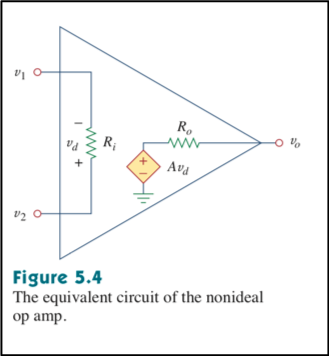
\includegraphics[width=0.5\textwidth]{figures/op-amp1}
\\
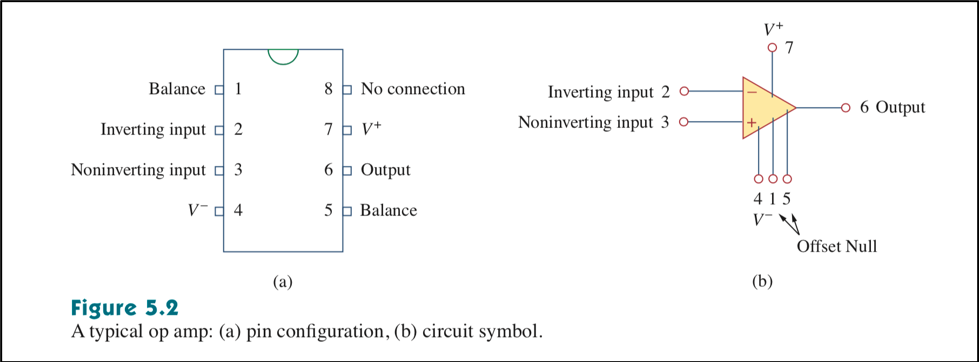
\includegraphics[width=\textwidth]{figures/op-amp2}

\begin{enumerate}
	\item Behaves like a voltage-controlled voltage source
	\item They can amplify, sum, subtract, multiply, differentiate, integrate
	\item They are active circuit elements
	\item Though they have somewhat more complicated internal workings, we typically represent them in electrical circuits as a triangle with three (sometimes five) very important terminals:
	\subitem An inverting input ($—$ sign, typically represented up top for convenience, but it need not be)
	\subitem A non-inverting input (+ sign, typically on bottom)
	\subitem An output
	\subitem A positive power supply
	\subitem A negative power supply
\end{enumerate}

\section{Some rules}
There are \textbf{three important features of ideal operational amplifiers} that we must understand thoroughly. These are things worth stamping in your brain.

\begin{enumerate}
	\item \textbf{Infinite open-loop gain.} The ``A'' of the gain is infinitely large such that any difference in voltages $V_1$ and $V_2$ causes an enormously large output voltage. As much as is being supplied. (The real value of gain in most operational amplifiers is between $10^{5}$ and $10^8$.)
	\item \textbf{Infinite input impedance.} Current cannot travel between the inverting and non-inverting terminals. (Really, the impedance is between $10^5$ and $10^13$ ohms and is often signal dependent.)
	\item \textbf{Zero output impedance.} There is no loss transmitting a voltage difference to the output. (Really is about 10-100 ohms and is chip dependent.)
\end{enumerate}

\section{Some conveniences}
\begin{enumerate}
	\item With infinite input impedance, no current can flow into or out of the terminals and hence $i_1$ and $i_2$ are equal to 0.
	\item Since no current flows across the terminals, the terminals are at equal potential. Hence ``$v_1 = v_2$''.
\end{enumerate}

\newpage
\section{Some examples}

\subsection{Inverting amplifier}
We will apply the conservation of mass at this point to solve our equations.  This is among the simplest and most effective ways to add gain to a circuit. So much so that you will use it again and again and again in life and especially in labs

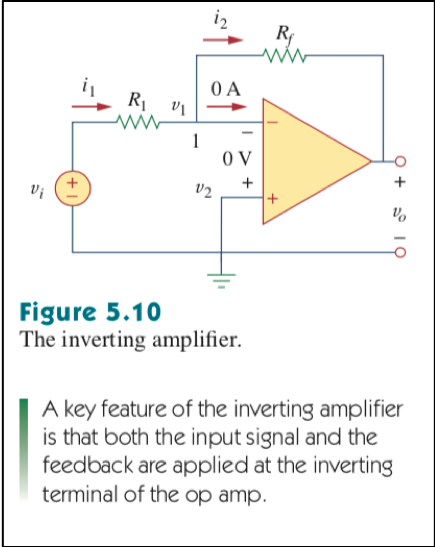
\includegraphics[width=0.5\textwidth]{figures/op-amp3}

We apply KCL at the node for v1
\begin{enumerate}

	\item Since the non-inverting amplifier is attached to the ground, $v_2 = 0$ 
	\item Using Rule 2 from earlier (Infinite Input Impedance) there is no current between v_1 and v_2. Therefore, $v_2 = v_1 = 0$
	\item From this we can conclude that $i_1 = i_2 = i$
	\item Using Ohm's Law ( $V = iR$) We can rewrite the equation in terms of current: $i = \frac{V}{R}
	\subitem $i_1 = \frac{v_i - v_1}{R_1}$
	\subitem $i_2 = \frac{v_1 - v_0}{R_f}$
	\item Using the known values from above, set the two current equations together and solve for $v_0$
	\subitem Known: $i_1 = i_2 = i$ and $v_2 = v_1 = 0$
	\subitem $ \frac{v_i - v_1}{R_1} = \frac{v_1 - v_0}{R_f}$
	\subitem $ \frac{v_i}{R_1} = \frac{-v_0}{R_f}$
	\subitem $v_0 = (\frac{-R_f}{R_1})*v_i $
	\item The gain factor is $\frac{R_f}{R_1}$

\end{enumerate}




\subsection{Non-inverting amplifier}
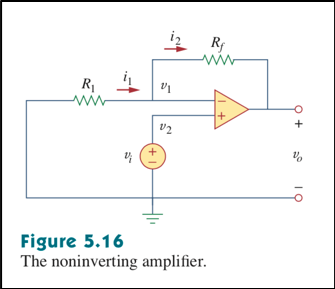
\includegraphics[width=0.5\textwidth]{figures/op-amp4}

Again, the name might imply what it does. It will amplify our input signal without inverting it.

We can again perform Nodal analysis.
\begin{enumerate}

	\item Since the non-inverting amplifier is attached to the ground, $v_2 = v_i$ 
	\item Using Rule 2 from earlier (Infinite Input Impedance) there is no current between v_1 and v_2. Therefore, $v_2 = v_1 = v_i$
	\item From this we can conclude that $i_1 = i_2 = i$
	\item Using Ohm's Law ( $V = iR$) We can rewrite the equation in terms of current: $i = \frac{V}{R}
	\subitem $i_1 = \frac{v_g - v_1}{R_1}$
	\subitem $i_2 = \frac{v_1 - v_0}{R_f}$
	\item Using the known values from above, set the two current equations together and solve for $v_0$
	\subitem Known: $i_1 = i_2 = i$, $v_g = 0$, and $v_2 = v_1 = v_i$
	\subitem $\frac{v_g - v_i}{R_1} = \frac{v_i - v_0}{R_f}$
	\subitem $\frac{-v_i}{R_1} = \frac{v_i - v_0}{R_f}$
	\subitem $v_0 = (1+ \frac{R_f}{R_1})*v_i$
	\item The gain factor is $1+ \frac{R_f}{R_1}$

\end{enumerate}



\subsection{Voltage follower}
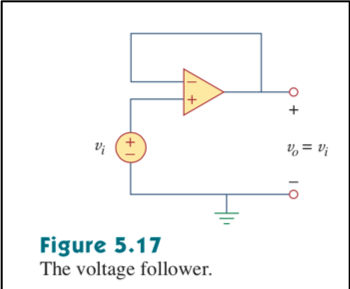
\includegraphics[width=0.5\textwidth]{figures/op-amp5.png}

What if we didn’t have any resistors? $\rightarrow$ Vi = v2 = v1 = Vo $\rightarrow Vi = Vo$

This is used to transfer voltage without transferring current. 



\subsection{Summing amplifier}
\subsection{Differential amplifier (as homework)}



\chapter{Circuit analysis: I. Nodal analysis}
01/22/2019
\section{Nodes and branches}
\section{Kirchhoff's Laws}
\subsection{Kirchhoff's Current Law}
\subsection{Kirchhoff's Voltage Law}
\section{Nodal analysis}
\section{Solving simultaneous equations}
\subsection{Cramer's Rule}



\chapter{Circuit analysis: II. Mesh analysis; Homework I}
01/24/2019
\section{Mesh analysis}
\section{Steps of mesh analysis}
\section{Writing mesh equations directly in matrix form}



\chapter{Circuit analysis: III. Supernodes and supermeshes}
01/29/2019 – Lecture 6. 
\section{Nodal analysis with an independent current source}
\section{Nodal analysis with voltage sources, \textbf{Supernodes}}
\section{Nodal analysis with controlled sources}
\section{Mesh analysis with current sources}
\section{Mesh analysis with controlled sources, \textbf{Supermeshes}}



\chapter{Circuit analysis: IV. Circuit theorems}
01/31/2019 – Lecture 7. 
\section{Circuit theorems}
\section{Linearity}
\section{Superposition}
\section{Source transformation}
\section{Thevenin equivalents}
\section{Norton equivalents}
\section{Equivalents with dependents}



\chapter{Circuit analysis: V. When to choose between analyses}
02/05/2019 – Lecture 8. 

\chapter{A review of the material thus far; Homework II}
02/07/2019 – Lecture 9. 

\section{How to measure voltage and current}

\chapter*{Exam I}
02/12/2019



\part{Systems}



\chapter{The Laplace Transform: I. What it is and why it is important}
02/14/2019 – Lecture 10. 
\section{How do we know our world looks like this?}
\section{Euler's identity / Euler's formula}
\section{The Laplace transform}
\section{The Laplace transform of 1}
\section{The $s$-plane}
\section{The linearity of the Laplace transform}
\section{The Laplace transform of $e^{at}$}
\section{The Laplace transform of $dx/dt$}
\section{The Laplace transform in RLC circuits}
\subsection{Resistors}
\subsection{Inductors}
\subsection{Capacitors}
\subsection{RLC}
\section{Two important places, zeros and poles}



\chapter{The Laplace Transform: II. How to use it}
02/19/2019 – Lecture 11. 
\section{The inverse Laplace transform}
\section{The Laplace transform of $\sin$}
\section{The Laplace transform of $t^n$}
\section{Some applicability}



\chapter{Circuits as ODEs: I. First-order}
02/21/2019 – Lecture 12. 
\section{Source-free RC circuits}
\subsection{One resistor, one capacitor}
\subsection{Two or more resistors and/or capacitors}
\section{Source-free ``active'' circuits}
\section{First-order systems with sources}
\section{Several singular functions}
\subsection{Unit step function, $u(t-t_0) = 1, t>t_0$}
\subsubsection{The Laplace transform of the unit step function}
\subsection{Unit impulse function, $\delta(t) = du(t)/dt$}
\subsubsection{Its ``sifting'' abilities}
\subsubsection{The Laplace transform of the unit impulse function}
\subsection{Unit ramp function, $r(t) = \int u(t)dt $}
\subsubsection{The Laplace transform of the unit impulse function}



\chapter{Circuits as ODEs: II. Second-order}
02/26/2019 – Lecture 13. 
\section{A series RLC circuit}



\chapter{System response: I. Convolution; Homework III}
02/28/2019 – Lecture 14. 
\section{An introduction to thinking in systems}
Viewing everything as a ``system''. 
\subsection{Domains of interest, of command}
\subsection{The time-domain, or: our typical realm}
\subsection{The frequency-domain, or: our new realm}
\subsection{The $s$-domain, or: our magical realm}
\section{Inputs and outputs}
\section{Somewhere in the between}
\section{Convolution in the time-domain}
\section{Multiplication in the frequency- and $s$-domain}



\chapter{System response: II. Stability}
03/12/2019 – Lecture 15. 
\section{An introduction}
\subsection{What do we mean by stability?}
\section{Undamped, $\zeta = 0$}
\section{Underdamped, $0 < \zeta < 1$}
\section{Overdamped, $\zeta > 1$}



\part{\& Signals}



\chapter{System response: III. The frequency domain}
03/14/2019 – Lecture 16. 



\chapter{System response: IV. Filters}
03/19/2019 – Lecture 17. 



\chapter{System response: V. Feedback; Homework IV}
03/21/2019 – Lecture 18. 



\chapter*{Exam II}
03/26/2019



\part{in Biomedical Engineering}



\chapter{Bioelectricity: I. Passive properties}
03/28/2019 – Lecture 19. 
\section{Modeling biological material with a simple circuit, $R_1 + (R_2||C)$}
\section{Resistance-Reactance Plane}
\section{What can we do with this information?}



\chapter{Bioelectricity: II. Active properties}
04/02/2019 – Lecture 20. 



\chapter{Bioelectricity: III. Measurement}
04/04/2019 – Lecture 21. 



\chapter{Digital circuits: I. Discretization}
04/09/2019 – Lecture 22. 



\chapter{Digital circuits: II. Logic; Homework V}
04/11/2019 – Lecture 23. 



\chapter{Happenstance: A few BME specific situations}
04/16/2019 – Lecture 24. 



\chapter{Circumstance: A few BME specific standards}
04/18/2019 – Lecture 25. 



\chapter{A philosophy of circuits, systems, and signals; Homework VI}
04/23/2019 – Lecture 26. 



\chapter*{Exam III}
04/26/2019 



\end{document}
